\subsection{Data}
The PhysioNet/CinC Challenge 2020 development set consisted of $43101$ ECG-recordings. The datasets were sourced from six subsets from four different sources:

\begin{itemize}
    \item The first source is China Physiological Signal Challenge 2018 which consists of two subsets: The original China Physiological Signal Challenge 2018 dataset \cite{liu_open_2018} and an extra set called China Physiological Signal Challenge Extra. 
    \item The second source is the Physikalisch-Technische Bundesanstalt (PTB) which consists of two subsets. The first one is the PTB Diagnostic \cite{bousseljot_nutzung_2009} and the second subset is PTB-XL \cite{wagner_ptb-xl_2020-1}
    \item The third source is the St. Petersburg Institute of Cardiological Technics (INCART) database \cite{goldberger_physiobank_2000}
    \item  The fourth is the Georgia 12-Lead ECG Challenge Database which is a new database and is still not described in any paper other than the PhysioNet/CinC Challenge 2020 paper \cite{alday_classification_2020}.
\end{itemize}
A total of $111$ different diagnoses were present in the total dataset. Each ECG-recording had at least one diagnosis, but some also had more than one diagnosis. The classification of such a dataset is considered to be a multi-label, multi-class classification problem. The goal of PhysioNet / CinC Challenge 2020 was to classify $27$ of the $111$ diagnoses. 



\subsubsection{Splitting of data}\hfill \break

The data were split into training (90\%) and validation (10\%) data using 10-fold stratified cross-validation with random state $=42$ \cite{pedregosa_scikit-learn_2011}. The stratification arranged the splitting such that the distribution of diagnoses was the same in both the train and validation data for each fold.

\subsection{Preprocessing data}
Initially, the diagnosis was encoded with Systematized Nomenclature of Medicine Clinical Terms (SNOMED-CT). The SNOMED-CT codes were decoded into human-readable diagnosis and one-hot encoded into a $27$-bit long array. Each of the bits in the array represented one of the $27$ scored diagnoses in the PhysioNet/CinC Challenge 2020 \cite{alday_classification_2020}. The $84$ unscored diagnoses were overlooked and did not represent any change in the 27-bit long label array. The same labels were used in both the CNN-models and the ensemble models, but the preprocessing and feature extraction from the ECG was done differently.

\subsubsection{Preprocessing for the convolutional neural networks} \hfill \break
All ECG-recordings used by the CNN-models were padded or truncated to a signal length of $5000$ samples. Padding and truncation were done by removing any parts longer than $5000$ samples and adding a tail of $5000 - n$ zeros to any recording of length $n<5000$. The rule-based model on the other hand, which was used in two of eight CNN-models, analyzed the ECG before padding or truncation to $5000$ samples.

The $27$ diagnoses/classes were not balanced and, to prevent the CNN-models to learn more from the diagnosis that occurred more frequently in the dataset, a class weight was calculated. The weights were fed to the models during training and gave higher priority to ECGs with rare diagnoses than diagnoses that occur more frequently in the dataset. 

\subsubsection{Preprocessing for the ensemble models}\hfill \break
All ECG recordings were fed into an ECG-featurizer function \cite{bjorn-jostein_singstad_ecg-featurizer_nodate}. The ECG-Featurizer analyzed the ECGs and extracted $112$ features from the ECGs. All of the $112$ features were used in the 12-lead classification while only $63$ were used in the 2-lead classification. Only features that were extracted from lead $II$ and V5 were used in the 2-lead model.

$42 720$ of $43101$ ECGs were successfully featurized by the ECG-featurizer. In addition, $146$ ECG-recordings were removed due to missing values. This gave a total dataset of $42574$ successfully  featurized ECGs to use by the ensemble models.


\subsection{Model architectures}
\subsubsection{CNN architectures}\hfill \break
The CNN architectures, used in this study, was the same as in \cite{bjorn-jostein_singstad_classifying_2020}. The models are listed in table \ref{tab:modelcombo}. The new contribution in this study is that the $8$ models were scored using cross-validation on the development data. \newline\newline

\vspace{4 mm}
\begin{table}[!htb]
        \centering
        \caption{The eight CNN models developed in \cite{bjorn-jostein_singstad_classifying_2020} and used in this study}
            \scalebox{1.0}{
                \begin{tabular}{lr} \hline\hline
                        Model     \\\hline
                        A) FCN                       \\
                        B) Encoder                   \\
                        C) FCN $||$ age, gender              \\   
                        D) Encoder $||$ age, gender       \\
                        E) Encoder $||$ FCN            \\
                        F) Ecoder $||$ FCN $||$ age, gender     \\
                        G) Encoder $||$ FCN + rule-based model      \\
                        H) Encoder $||$ FCN $||$ age, gender + rule-based model    \\\hline\hline
                \end{tabular}}
                \label{tab:modelcombo}
\end{table}
\vspace{4 mm}
\newline

\subsubsection{Ensemble model architecture}\hfill \break
The models trained on the featurized ECG-data were build using scikit-multi learn \cite{szymanski_scikit-multilearn_2019}. Scikit-multi learn is a library used for multi-label classification. The ensemble models were built using label space partitioning classifiers \cite{szymanski_how_2016}, classifier chains \cite{read_classifier_2009} and random forests. The label space partitioning classifier is a clustering algorithm where each cluster is a separate classification problem. The clusters were selected using a method called fixed label space clusterer. This method lets the developer define the clusters. The clusters in this study were created by iterating over all diagnosis in the training set and for the $n$-th diagnosis, there was $m_n$ diagnosis that co-existed with the $n$-th diagnosis across the data set. In total there were $27$ clusters and the size of the clusters, $m_n + 1$, were different for each of the folds in the 10-folded cross-validation. This is illustrated in figure \ref{fig:diagnosis_co_exist}.

\begin{figure}[!hbp]
    \centering
    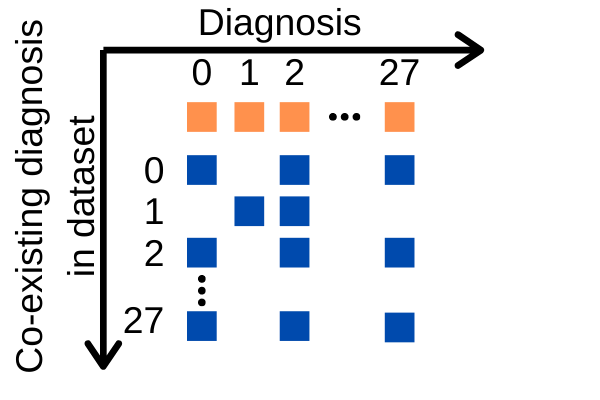
\includegraphics[width=.6\textwidth]{Figures/Diagnosis_cluster_axis.png}
    \caption{The figure shows how each of the 27 diagnoses co-existed with one or more of the other 26 diagnoses when looking across the whole development dataset. The 27 clusters that were used for the ensemble models used the same index as the co-existing diagnosis.}
    \label{fig:diagnosis_co_exist}
\end{figure}



\subsection{Threshold optimization}
The CNN-models needed prediction thresholds for the 27 classes to classify. New thresholds were set for each fold. A method called Nelder-Mead downhill simplex method \cite{nelder_simplex_1965, virtanen_scipy_2020} was used to optimize the thresholds individually with PhysioNet/CinC Challenge score as the optimization goal. This method can be computationally heavy and therefore a subset of the training set was used to optimize the threshold. The subset was determined using a stratified 10-fold and then selecting the first validation fold as the threshold optimization set.

The Nelder-Mead downhill simplex method is used to find the local minimum of a function using the function itself and an initial guess of the optimal variable of the function. In the first fold of the 10-folded cross-validation, the initial guess for the Nelder-Mead optimization algorithm was found by giving a 27-element long array values of ones and multiplied it with a variable that was given values from 0 to 1, with a step size of 0.05. The next folds in the 10-folded cross-validation used the threshold found by the Nelder-Mead optimization algorithm in the previous fold as the initial guess. 

The Ensemble models on the other hand did not need any threshold optimization  as the output was binarized by the model.





\subsection{Explanation models}
To add explainability to the models used in this study a local interpretable model-agnostic explanation (LIME) was used \cite{ribeiro_why_2016}. LIME explains the features importance, locally, for a given prediction. LIME uses a linear model to explain the prediction of the complex CNNs and ensemble models used in this study. As a proof-of-concept for such explanation models, the 12-lead ensemble model and the CNN encoder model were selected to be explained. The ensemble model was explained using a tabular explainer-function.

To explain the CNN model an explainer called recurrent explainer was used. The Encoder model was simplified by swapping the last layer in the Encoder-model with a softmax-layer with two nodes and the dataset was modified such that normal sinus rhythm was equal to normal class and all other diagnoses were equal to abnormal class.

\newpage
